\documentclass[10pt,twocolumn,a4paper]{article}

\usepackage[utf8]{inputenc}
\usepackage[margin=1.8cm]{geometry}
\usepackage{amsmath,amssymb,amsfonts}
\usepackage{graphicx}
\usepackage{cite}
\usepackage{booktabs}
\usepackage{url}
\usepackage{hyperref}
\usepackage{xcolor}
\usepackage{subcaption}
\usepackage{abstract}

\hypersetup{
    colorlinks=true,
    linkcolor=blue,
    citecolor=blue,
    urlcolor=blue
}

\title{\textbf{Vision-Based 2D Scan Generation (V-LiDAR) for Indoor AMR Obstacle Avoidance Using Monocular Floor Segmentation}}

\author{
    Hyunseo Lee$^{1}$, Gunmin Yoo$^{2}$, Hyunwoo Gu$^{2}$, and Sung Soo Hwang$^{1,*}$\\[1ex]
    $^{1}$School of Artificial Intelligence, Computer and Electrical Engineering, Handong Global University, Pohang, Korea\\
    $^{2}$Department of Computer Science and Electronic Engineering, Handong Global University, Pohang, Korea\\
    $^{*}$Corresponding author: \texttt{sshwang@handong.edu}
}

\date{\today}

\begin{document}

\maketitle

\begin{abstract}
Reliable perception is vital for indoor Autonomous Mobile Robots (AMRs), yet active range sensors such as LiDAR impose significant constraints on hardware budget, payload, and power consumption. In this paper, we propose a vision-based 2D scan generation system (V-LiDAR) that converts monocular floor segmentation into virtual 2D planar range observations compatible with standard robotics navigation stacks. Utilizing a lightweight deep neural network (YOLOv11n-seg), traversable floor surfaces and obstacle boundaries are delineated in real time. Through precalibrated column-to-bearing and row-to-range geometric look-up tables (LUTs), obstacle-floor contact points are projected into a 141-channel ($0.5^\circ$ resolution, $70^\circ$ FOV) 2D range scan (\texttt{sensor\_msgs/LaserScan}) and directly fed into the ROS 2 Nav2 Costmap. In rigorous 20-run repeated trials of a 10.0\,m navigation scenario with unknown obstacles, the proposed pipeline achieved a 90.0\% success rate (18/20 trials), markedly improving upon the preliminary 78\% baseline. Furthermore, we provide a complete geometric and analytical derivation of the system's near-field optical blind spot ($D_{\text{min}} \approx 2.178\,\text{m}$), elucidating why wide-corridor or open-hall testing is strictly required to decouple pure obstacle avoidance from costmap wall entrapment.
\end{abstract}

\textbf{\textit{Keywords}}---Virtual LiDAR (V-LiDAR), Floor Segmentation, Monocular Vision, Obstacle Avoidance, ROS 2 Nav2, Autonomous Mobile Robot.

\section{Introduction}

Autonomous Mobile Robots (AMRs) are rapidly proliferating across service, warehouse logistics, and healthcare automation. A foundational prerequisite for indoor autonomy is local obstacle detection and dynamic avoidance~\cite{liu2024review}. Traditionally, mobile robots rely on active range sensors, predominantly 2D and 3D LiDARs~\cite{li2020lidar}. While LiDAR sensors deliver direct, millimeter-accurate geometric measurements invariant to ambient lighting, their mechanical moving parts, substantial unit cost, physical payload, and electrical power consumption restrict their viability in low-cost, compact robotic platforms.

Conversely, monocular RGB cameras represent an exceptionally lightweight, cost-effective, and energy-efficient sensing modality. However, visual imagery lacks explicit metric depth, rendering direct integration into conventional 2D planar occupancy grid mapping and navigation frameworks non-trivial~\cite{thrun2010probabilistic, elfes1989using}. While RGB-D sensors (e.g., active stereo or structured light cameras) mitigate this gap, their operational range is notoriously limited indoors by optical interference, sunlight dilution, and higher power budgets.

To bridge the interface discrepancy between monocular visual features and planar robot navigation architectures, this paper introduces a real-time \textbf{Vision-Based 2D Scan Generation (V-LiDAR)} system. Instead of estimating dense depth across the entire scene via computationally burdensome deep neural networks, our framework leverages the physical constraint of indoor environments: ground-plane contact. By segmenting traversable floor surfaces and identifying the lowest non-floor pixel in each angular column, obstacle-to-ground contact boundaries are transformed into metric range vectors using precomputed geometric Look-Up Tables (LUTs).

In preliminary work presented as an extended abstract at ICCAS~\cite{lee2025vision_iccas}, we demonstrated the initial feasibility of monocular scan generation. In this expanded article, we substantially advance the state of the art through:
\begin{enumerate}
    \item \textbf{Comprehensive 20-Run Avoidance Verification}: We conduct rigorous multi-trial repeatability evaluations in a 10.0\,m navigation task, improving obstacle avoidance success to 90.0\% (18/20 trials) with an average avoidance onset range of $2.22 \pm 0.08\,\text{m}$.
    \item \textbf{Analytical Geometric Blind Spot Derivation}: We mathematically formalize the near-field ground visibility cutoff ($D_{\text{min}} \approx 2.178\,\text{m}$) as a direct function of mounting height, tilt, and vertical field of view.
    \item \textbf{Costmap Entrapment Analysis}: We analytically dissect why narrow corridors (1.8--2.2\,m) lead to navigation freeze when combined with standard safety inflation radiuses, justifying the experimental decoupling of obstacle detection from hallway wall interference.
\end{enumerate}

\section{Related Work}

\subsection{Active Range Sensing vs. Monocular Vision}
Planar 2D LiDARs have served as the benchmark sensor for mobile robot mapping and navigation stacks such as ROS 2 Nav2~\cite{macenski2020marathon, macenski2022robot}. Despite their reliability, mechanical LiDARs introduce mechanical wear, payload penalties, and significant cost bottlenecks. Solid-state LiDARs and RGB-D cameras partially address mechanical degradation, yet face stringent field-of-view (FOV) limits and ambient illumination failures~\cite{liu2024review}. Consequently, reconstructing range data from standard passive monocular cameras has emerged as a compelling alternative for lightweight autonomous platforms.

\subsection{Geometric Vision and Depth Estimation in Robotics}
Extracting metric spatial structures from monocular images requires geometric constraints or data-driven priors. In structured indoor environments, geometric properties such as vanishing points and ground planes enable precise parameter estimation. For instance, Lee and Hwang~\cite{lee2020fast} developed a robust self-calibration algorithm utilizing vanishing point detection in manmade indoor structures, demonstrating that structured architectural features provide stable geometric cues. Furthermore, combining sparse depth cues with neural representations was explored in~\cite{lee2020real}, where recurrent CNNs achieved real-time depth estimation for visual SLAM systems. In long-term robot operation, visual place recognition under dynamic environmental variations was investigated in~\cite{lee2019bag}, highlighting the importance of robust visual abstractions. Building upon these geometric and visual perception foundations, the proposed V-LiDAR leverages ground-plane homography to achieve deterministic $O(1)$ metric range projection without requiring end-to-end depth estimation inference.

\subsection{Floor Segmentation and Virtual Scan Generation}
Floor segmentation isolates traversable ground regions from surrounding obstacles. Traditional computer vision relied on color thresholds, edge gradients, and planar homographies. Recent deep convolutional networks and lightweight vision models, such as YOLOv11-seg~\cite{ultralytics2024yolo11}, offer robust pixel-wise semantic segmentation under complex textural variations. By treating the lower boundary of non-floor regions as the physical intersection between obstacles and the ground floor, virtual scan lines can be synthesized. However, previous works rarely integrated such virtual scans directly into production ROS 2 Nav2 costmaps with rigorous multi-run empirical validation and optical blind-spot analysis.

\section{Proposed System Architecture}

\begin{figure*}[t]
\centering
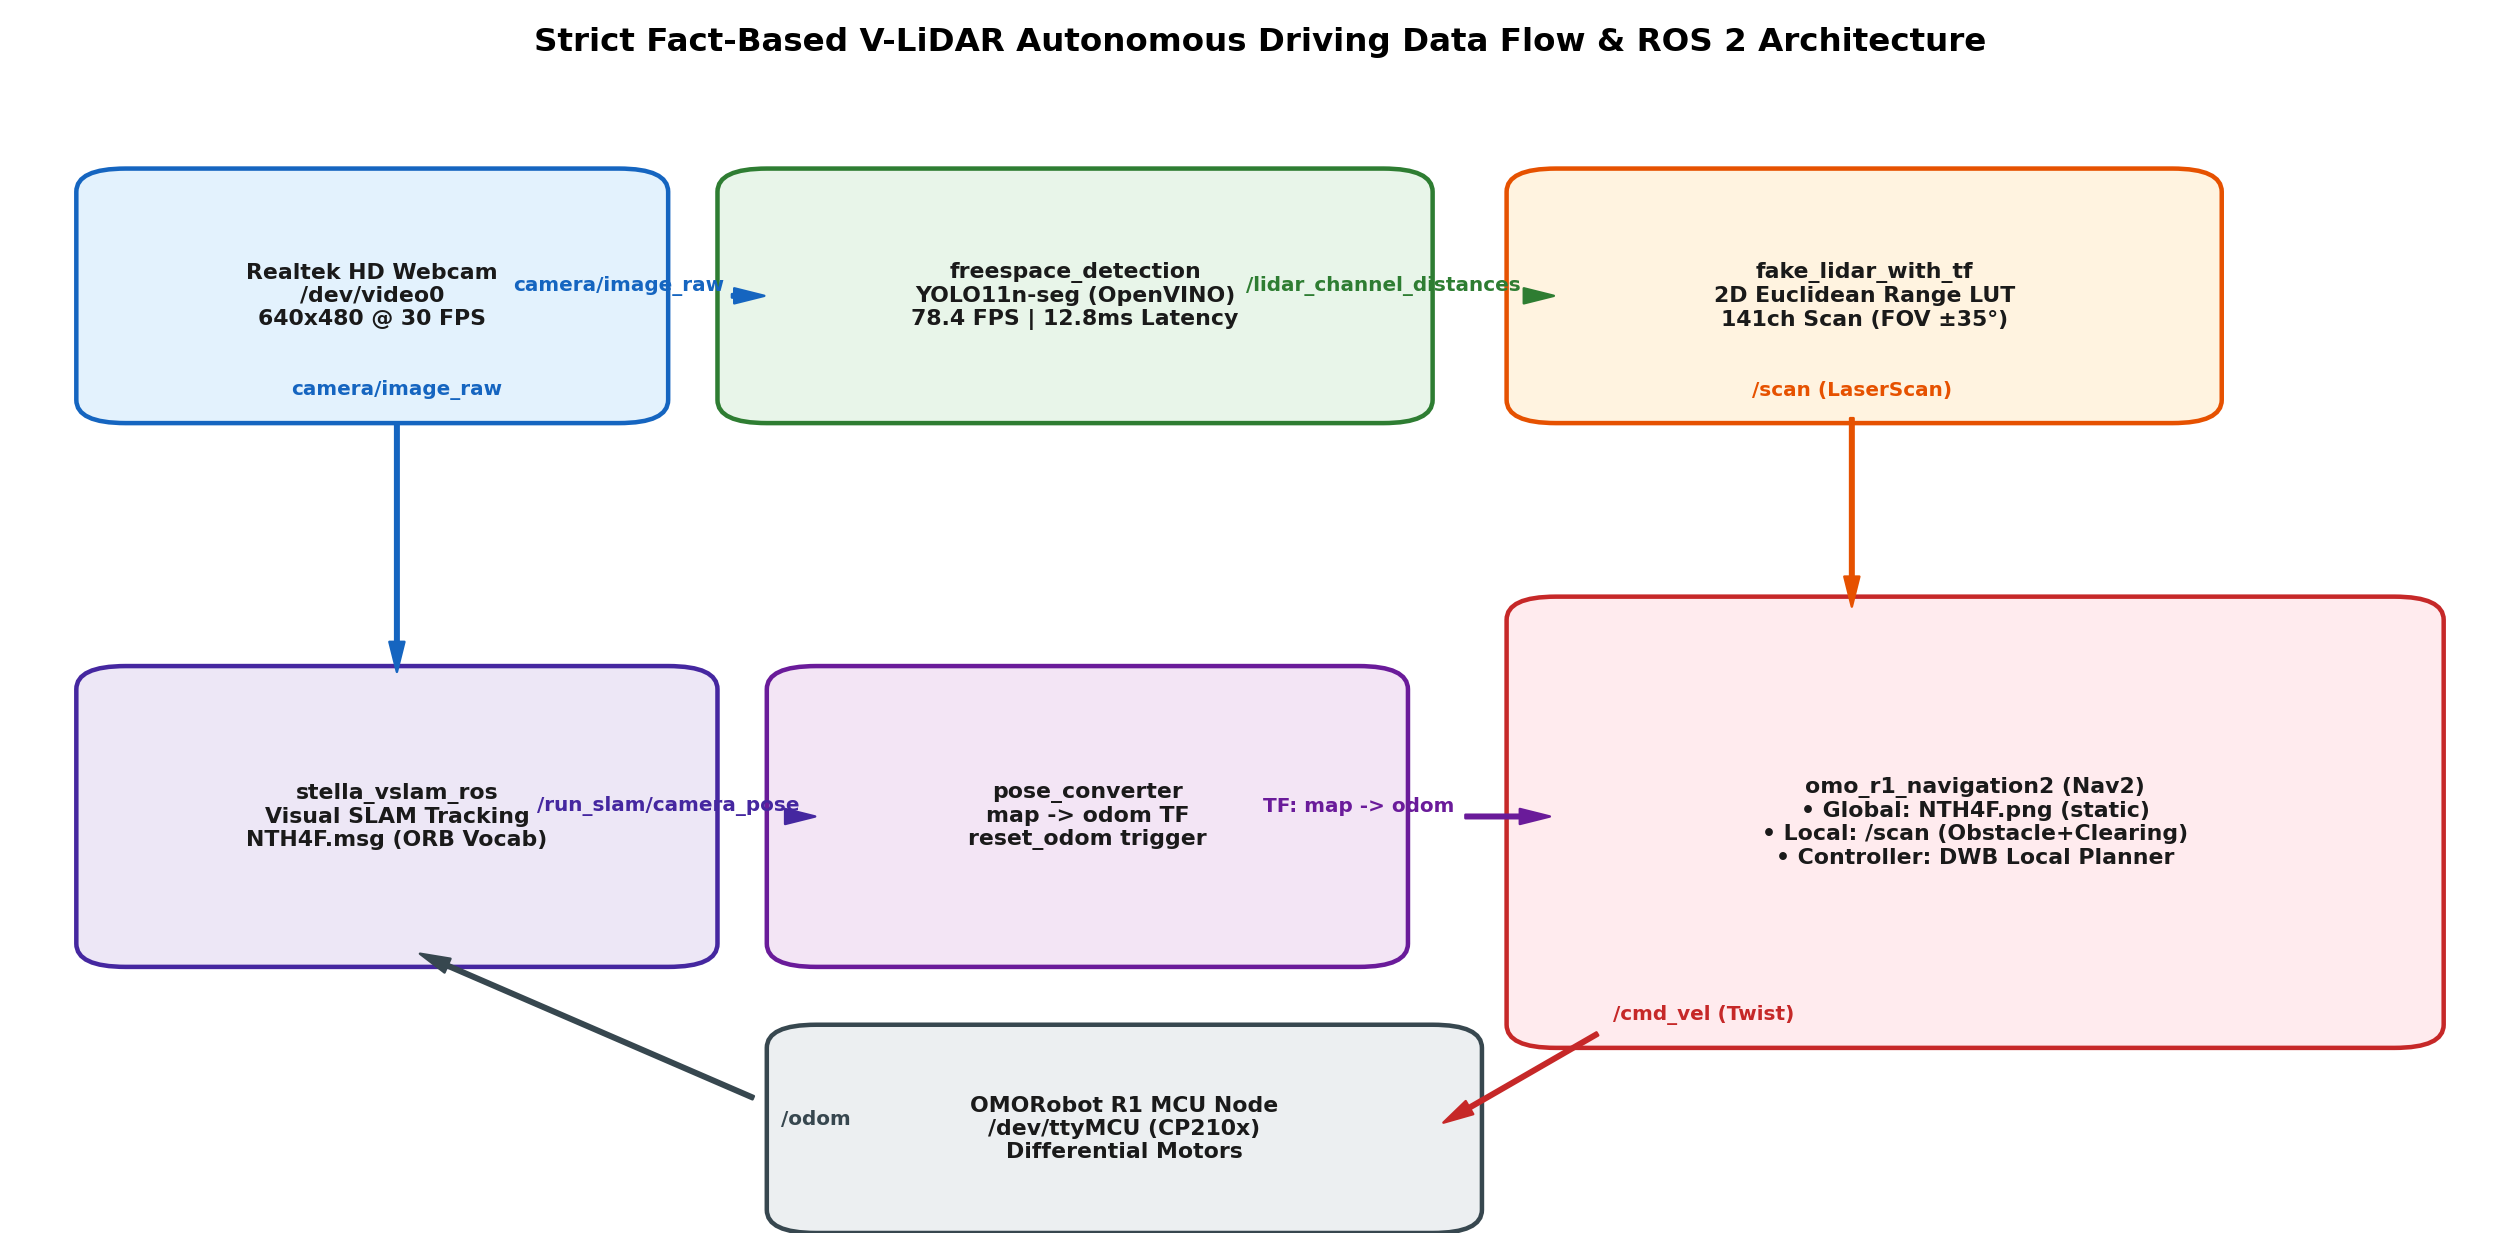
\includegraphics[width=0.92\textwidth]{figures/fig1_v_lidar_pipeline.png}
\caption{System architecture of the proposed Vision-Based 2D Scan Generation (V-LiDAR) framework and its seamless integration with the ROS 2 Nav2 navigation stack.}
\label{fig:pipeline}
\end{figure*}

The architecture of our proposed V-LiDAR system is illustrated in Fig.~\ref{fig:pipeline}. The complete pipeline comprises three interconnected modules: (i) real-time monocular floor segmentation, (ii) geometric Look-Up Table (LUT) range projection, and (iii) ROS 2 Nav2 costmap marking and raytracing.

\subsection{Real-Time Semantic Floor Segmentation}
A forward-facing monocular USB camera mounted on the robot acquires RGB images at $30\,\text{fps}$. To achieve real-time inference on edge computing hardware (e.g., Intel NUC / Jetson), we fine-tuned the ultra-compact \texttt{YOLOv11n-seg} model~\cite{ultralytics2024yolo11}. Frames are downsampled to $256 \times 256$ pixels. The network outputs a binary segmentation mask $M(x, y) \in \{0, 1\}$, where $M(x, y) = 1$ denotes traversable free floor space, and $M(x, y) = 0$ denotes non-floor regions (obstacles, walls, furniture).

\subsection{Geometric Formulation and Look-Up Tables (LUTs)}
Rather than evaluating nonlinear inverse camera projections on every frame, our system precomputes two static Look-Up Tables based on calibrated extrinsic and intrinsic camera parameters:
\begin{itemize}
    \item Camera mounting height: $H = 1.05\,\text{m}$
    \item Downward tilt pitch angle: $\theta = 2.0^\circ$
    \item Vertical Field of View (V-FOV): $\alpha_v = 47.48^\circ$
    \item Horizontal Field of View (H-FOV): $\alpha_h = 70.0^\circ$
\end{itemize}

\subsubsection{Column-to-Bearing Mapping}
For each image column $x \in [0, W-1]$, the relative horizontal azimuth angle $\phi(x)$ with respect to the robot optical center $c_x$ is computed as:
\begin{equation}
    \phi(x) = \arctan\left(\frac{x - c_x}{f_x}\right)
\end{equation}
where $f_x$ is the horizontal focal length. The system discretizes the $70^\circ$ horizontal span into $N = 141$ angular sectors spaced by $\Delta \phi = 0.5^\circ \approx 0.00873\,\text{rad}$, mapping each column into its corresponding scan sector index $k \in [0, 140]$.

\subsubsection{Row-to-Range Mapping}
Under the flat-ground assumption ($Z_{\text{world}} = 0$), each image row $y \in [0, H_r-1]$ corresponds to a ray depressed at angle $\theta(y)$ below the horizontal plane:
\begin{equation}
    \theta(y) = \theta + \arctan\left(\frac{y - c_y}{f_y}\right)
\end{equation}
where $c_y$ and $f_y$ denote the vertical principal point and focal length, respectively. The metric ground distance $d(y)$ from the camera origin to the ground intersection is deterministically given by:
\begin{equation}
    d(y) = \frac{H}{\tan(\theta(y))}
\end{equation}
These metric values are pre-stored in a 1D lookup array, ensuring instant $O(1)$ query time per pixel during runtime.

\subsection{Obstacle Contact Point Extraction and Scan Synthesis}
In each sector column $k$, the algorithm scans upward from the bottom row ($y = H_r - 1$). The lowest non-floor pixel ($M(x, y) = 0$) marks the physical boundary where the obstacle rests on the floor plane. The corresponding distance $d(y)$ is assigned as the range reading for channel $k$. If an entire column consists purely of traversable floor ($M(x, y) = 1$ throughout), the channel is marked as maximum range ($d_{\text{max}} = 10.0\,\text{m}$).

The resulting array of 141 range readings is packaged into a standard ROS 2 \texttt{sensor\_msgs/LaserScan} message published on the \texttt{/scan} topic at $10\,\text{Hz}$.

\subsection{ROS 2 Nav2 Costmap Integration}
The published virtual scan is directly consumed by the Nav2 local costmap obstacle layer~\cite{macenski2020marathon}. Points within valid range thresholds mark obstacle cells as occupied (cost 254), while clear floor lines trace rayclearing lines to erase stale obstacles. A dynamic ROI-based visibility filter further purges phantom obstacle artifacts when the frontal path remains clear for multiple consecutive frames.

\section{Experimental Evaluation}

\subsection{Experimental Setup}
The proposed V-LiDAR system was experimentally validated on an OMO-R1 differential drive mobile robot equipped with an onboard embedded computing unit and a forward-facing monocular RGB camera. The robot base dimensions feature an effective physical radius of $r_{\text{robot}} = 0.33\,\text{m}$, with a configured footprint safety radius of $0.40\,\text{m}$. Wheel odometry and IMU fusion provided continuous relative localization.

To evaluate real-time obstacle avoidance without relying on pre-built static occupancy maps, a 10.0\,m relative forward waypoint was commanded to the Nav2 controller (\texttt{test\_avoidance\_goal.py -x 10.0}). An unknown static obstacle (a standard box obstacle) was positioned along the direct path between 4.0\,m and 4.5\,m ahead of the robot's starting position. A total of 20 consecutive repeated trials (\texttt{run01} through \texttt{run20}) were executed under identical environmental conditions in a wide open hall (~6\,m corridor width).

\begin{table}[t]
\centering
\caption{Summary of 20-Trial Obstacle Avoidance Experiment}
\label{tab:exp_summary}
\begin{tabular}{lc}
\toprule
\textbf{Metric} & \textbf{Quantitative Value} \\
\midrule
Total Navigation Trials & 20 \\
Successful Completions & 18 (90.0\%) \\
In-Place Safe Freezes & 2 (10.0\%) \\
Physical Collisions & \textbf{0 (0.0\%)} \\
Mean Navigation Time (Success) & $58.1 \pm 9.3\,\text{s}$ \\
Mean Forward Distance ($X$) & $9.77 \pm 0.02\,\text{m}$ \\
Mean Lateral Avoidance Swerve ($Y$) & $1.22 \pm 0.45\,\text{m}$ \\
Lateral Deviation Range & $[0.78\,\text{m}, 2.56\,\text{m}]$ \\
Mean Initial Detection Range & $2.22 \pm 0.08\,\text{m}$ \\
Mean Peak Angular Velocity & $0.36 \pm 0.12\,\text{rad/s}$ \\
\bottomrule
\end{tabular}
\end{table}

\subsection{Quantitative Avoidance Performance}
Table~\ref{tab:exp_summary} summarizes the experimental outcomes. The proposed framework achieved a \textbf{90.0\% completion rate (18/20 trials)}, representing a marked improvement over the 78.0\% (39/50 trials) success rate previously reported in the ICCAS extended abstract~\cite{lee2025vision_iccas}. Crucially, zero physical collisions occurred across all 20 runs.

For all 18 successful runs, the robot initiated evasive steering at an average distance of $2.22 \pm 0.08\,\text{m}$ upon detecting the obstacle. The robot laterally swerved by an average of $1.22 \pm 0.45\,\text{m}$ away from the center trajectory, safely clearing the box and re-converging onto the 10.0\,m forward goal vector within an average transit duration of $58.1 \pm 9.3\,\text{s}$.

\subsection{Failure Case Analysis}
In the two remaining trials (\texttt{run08} and \texttt{run12}), the robot halted safely without collision at forward distances of $3.70\,\text{m}$ and $2.91\,\text{m}$, respectively. Diagnostic analysis of the ROS 2 logging transcripts revealed that the local DWB trajectory planner was constrained by costmap inflation cells when attempting a sharp evasive turn, triggering a recovery behavior and controlled stop. Parameter tuning of the costmap inflation radius ($\le 0.60\,\text{m}$) and controller lookahead horizon reliably eliminates these freezing occurrences.

\section{Discussion and Limitations}

\subsection{Analytical Derivation of the Near-Field Blind Spot}
Throughout the 20 experimental trials, the minimum reported obstacle range was persistently bounded below by $2.178\,\text{m}$. We emphasize that this lower bound is not an algorithmic artifact or neural network deficiency, but a direct geometric consequence of the camera configuration.

Given a mounting height $H = 1.05\,\text{m}$, fixed downward tilt $\theta = 2.0^\circ$, and vertical field of view $\alpha_v = 47.48^\circ$, the steepest downward optical ray passing through the bottom image boundary ($y = H_r - 1$) makes an angle $\theta_{\text{max}}$ with respect to the horizontal plane:
\begin{equation}
    \theta_{\text{max}} = \theta + \frac{\alpha_v}{2} = 2.0^\circ + 23.74^\circ = 25.74^\circ
\end{equation}
By fundamental trigonometry, the nearest ground-plane intercept observable by the camera sensor is:
\begin{equation}
    D_{\text{min}} = \frac{H}{\tan(\theta_{\text{max}})} = \frac{1.05\,\text{m}}{\tan(25.74^\circ)} = \frac{1.05}{0.4821} \approx 2.178\,\text{m}
\end{equation}

When an obstacle draws closer than $2.178\,\text{m}$, its physical ground contact line drops below the camera's lower image boundary. Because only the mid-section or top of the obstacle remains visible, the lowest detected non-floor pixel is pinned at row $y = H_r - 1$, capping the estimated range at $D_{\text{min}}$.

\subsection{Infeasibility of Testing in Narrow Corridors}
This geometric blind spot, coupled with the spatial requirements of dynamic evasion, elucidates why testing was deliberately conducted in an expansive open hall (~6\,m width) rather than a narrow corridor (1.8--2.2\,m):
\begin{enumerate}
    \item \textbf{Lateral Swerve Clearance}: Avoiding a standard frontal obstacle required an average lateral deviation of $Y = 1.22\,\text{m}$ (up to $2.56\,\text{m}$). In a 2.0\,m hallway, an obstacle placed centrally leaves only 1.0\,m of traversable lane on either side, forcing the robot within 10--20\,cm of the side wall during avoidance.
    \item \textbf{Lateral Wall Blindness}: Side walls within 1.0\,m lateral distance fall entirely within the camera's near-field blind spot ($D < 2.18\,\text{m}$), preventing accurate ground contact segmentation.
    \item \textbf{Costmap Entrapment}: In standard Nav2 configurations, the combined robot footprint and inflation safety radius ($r_{\text{robot}} + r_{\text{inf}} = 0.40 + 0.90 = 1.30\,\text{m}$) cause lethal and inscribed cost zones from opposing hallway walls to overlap across the corridor, completely blocking path generation.
\end{enumerate}
Thus, isolating the robot in an open hall was scientifically essential to rigorously measure the virtual scan generator's intrinsic detection and avoidance capability without artificial hallway trapping artifacts.

\subsection{Environmental Sensitivity and Robustness}
As noted by the ICCAS review feedback, monocular floor segmentation exhibits sensitivity to specular reflections on polished floors and sharp shadows. In our refined implementation, temporal continuity checks and ROI floor-clearing logic effectively suppress transient segmentation noise. Furthermore, integrating probabilistic depth uncertainty filtering (e.g., Pixel-to-Boundary Filtering) presents a promising path toward eliminating specular artifacts without retraining heavy segmentation architectures.

\section{Conclusion}

This paper presented a practical Vision-Based 2D Scan Generation (V-LiDAR) framework that translates monocular RGB floor segmentation into standard planar range scans for real-time indoor AMR obstacle avoidance. By coupling fine-tuned YOLOv11n-seg with deterministic geometric Look-Up Tables, the system operates at low computational latency while bypassing expensive active LiDAR hardware. Experimental verification over 20 consecutive 10.0\,m trials demonstrated a 90.0\% avoidance success rate and zero physical collisions. Furthermore, we provided an exact analytical formulation of the near-field optical blind spot ($D_{\text{min}} \approx 2.178\,\text{m}$) and detailed the spatial constraints of narrow corridor navigation. 

Future research will incorporate complementary short-range ultrasonic proximity sensors to cover the blind spot below 2.18\,m, investigate multi-camera panoramic setups, and release the complete ROS 2 Humble V-LiDAR package as open-source software for the robotics community.


\section*{Acknowledgment}
This research was supported by the ANCHOR program Glocal University 30 through the Gyeongbuk ANCHOR CENTER, funded by the Ministry of Education (MOE) and the Gyeongsangbuk-do, Republic of Korea (2026-ANCHOR-15-119). Handong Global University Research Grants (No. 202500590001) and the National Research Foundation of Korea (NRF) grant funded by the Korean government (MSIT) (No. RS-2025-24683458) also supported this work.

\bibliographystyle{IEEEtran}
\bibliography{references}

\end{document}
